\chapter{Exploratory Data Analysis}
\label{ch:eda}
\vspace{2em}

The following chapter discusses exploratory and analysis of AIS data using statistics and visualization. To start off, we first explain about AIS features description. We continue with AIS data exploration using statistics and visualization, which include erroneous value identification, and trajectory overview. 

\section{Data Description}
Looking back to the Introduction chapter, the typical AIS data packet is encoded as follows: \texttt{!AIVDM,1,1,,B,177KQJ5000G?tO`K>RA1wUbN0TKH,0*5C}. Each field is separated by a comma as there are 7 fields in the packet. Field 1 to 5 together with field 7 are specific to the encoding configuration of the data packet to enclose the actual message in field 6. From now on we will call field 6 as AIS payload.

The data in AIS payload is an ASCII-encoded bit vector. Each character represents 6-bits of data from which can be recovered by subtracting 48 to its ASCII value. If the result is greater than 40, subtract again with 8 \cite{aivsprotocolraymond}. For instance, the 6-bits interpretation of the first 4 characters in the above AIS payload is \texttt{000001 000111 000111 011011}. By concatenating all 6-bits representation of each AIS payload character, we end up with binary payload of the data. The first 6 bits of the binary payload are the message type. There are 27 message types in total, but in practice the most common types emit by AIS transmitter are 1, 3, 4, 5, 18, and 24 \cite{aivsprotocolraymond}. Type 1, 3, 4, and 18 transmit position-related information while type 5 and 24 transmit static and voyage related information. In normal operation, an AIS transceiver broadcasts a new position-related message every 2 to 10 seconds while underway and every 3 minutes while stationary. Besides, a new static message is sent every 6 minutes. The periodicity of the AIS message mentioned above does not happen in a real case. Most of the time the data is erroneous and irregular. We will discuss how to handle erroneous data later in the chapter.

Typically the amount of AIS data received from Singapore Straits contains 4 to 5 million records every month. The number could jump to 1 million records in a single busy day, but only 13,000 to 50,000 records on a quiet day. The last 10 days of the month are usually the busiest. Dynamic AIS message shares a common reporting structure for navigational information of total of 168 bits occupying AIS binary payload \cite{aivsprotocolraymond}. We will start by discussing every field in the AIS message. In general, every field belongs to either one of 3 categories, dynamic information, static information, and voyage-related information. The following list is part of dynamic information. Maritime Mobile Service Identity (MMSI) is a unique 9-digits identifier of AIS transceiver which usually stays in the vessel. Although MMSI is an AIS identifier, we could however use MMSI to identify a specific vessel. Navigational Status indicates vessel navigation activity around the sea. It explains whether a vessel is currently underway using engine, stationary at anchor, engaged in fishing, or other activities.

Rate-of-turn is values reported in degrees per minute between 0 to 708 which indicates the actual value of turning's rate of the vessel. Rate-of-turn in AIS message is encoded with a range of value from 0 to 128 whereby 0 means the ship is not turning whilst the plus-minus sign indicates the ship is turning right or left respectively. Given a rate-of-turn input (ROTin) from AIS message one can decode the actual ROT value by the following formula: ROT = 4.733 * SQRT(ROTin) degrees/min. Speed Over Ground (SOG) is the speed of the vessel relative to the surface of the earth. In the maritime world, there is another type of speed called Speed Over Water which is measured to water. The difference is speed-over-ground takes the speed of current into account which makes the total speed increase when the current flows in the same direction as the vessel and decreases when it flows astern, as opposed to speed-over-water that remains the same regardless of the current situation. AIS message's value for speed-over-ground is in 0.1 knot resolution from 0 to 102 knots, 1023 for not being available, and 1022 for speed over 102.2 knots.

Position accuracy is a 1-bit field in the AIS message to indicate if the vessel uses a DGPS sensor (value 1) or GNSS sensor (value 0, default) for the positioning system. The position accuracy of DGPS is less than 10m while GNSS is more than 10m. To ensure that ship information being transmitted is correct and up to date, the shipowner shall validate the data regularly per month or voyage whichever shorter. However, the accuracy of the ship sensors into AIS would not be checked. The shipowner shall conduct a separate check during the voyage to validate the accuracy \cite{imo1998}. Longitude and Latitude is one of the most useful information in trajectory prediction. Longitude and Latitude's value in the AIS message is given in minute/10000 unit. The primary unit for longitude and latitude is in degree from -180 (west) to 180 (east) and -90 (west) to 90 (east) respectively, so we need to divide the original number with 600000 to convert them into a degree. Course Over Ground (COG) is the angle relative to true north ranging from 0 to 359 with 0.1 degree resolution. Heading or bearing is the magnetic compass angle indicated during voyage ranging from 0 to 359 degree value with value 511 means not available.

The second cluster of AIS fields is static information. Static and dynamic information share a few attributes in common such as timestamp, MMSI, and message type. IMO number, Callsign, and Ship Name primarily have the same function to uniquely identify the vessel. IMO number contains the 3 letters "IMO" followed by 7-digit-number which consists of 6 digits unique number and 1 last digit to verify the integrity of IMO number. This is done by multiplying each digit by a factor of 2 to 7 corresponding to their position from right to left. For instances, IMO 9074729: (9x7)+(0x6)+(7x5)+(4x4)+(7x3)+(2x2) = 139. In this case the IMO number is verified as both are the same (Vuori, 2013). A Callsign number is a 6-digit alphanumeric identity that is assigned by a national licensing authority to a vessel and acts in the same way as a registration number for a vehicle. The first 2 alphanumeric prefix of callsign number refers to nationality of the vessel and followed by 2 or 3 alphanumeric digits. The prefix for Singapore's licensed stations is '9V'. The last vessel identification system is the ship name. Each ship name may consist of multiple MMSI and IMO numbers, therefore it's not recommended to use ship name only for vessel identification purposes. Ship Type in AIS is encoded in 0 to 99. The most common ship type is cargo, tanker, passenger, fishing, and tug vessel. Another static information is the dimension of 4 sides of the ship including bow, stern, port and starboard measured in meters. 

The last cluster in AIS fields is voyage-related information. Draught or Draft is the distance from the waterline to the hull of the vessel. Draught value ensures a safe balance of the maximum load of the vessel to operate on a voyage. Estimation Time Arrival as the name suggests is an estimated number of vessels to arrive in a month, day, hour, and minute to a Destination. In practice, the information in Destination and ETA is not reliable, as it has to be manually updated by humans rather than gather automatically by sensors \cite{aivsprotocolraymond}. Such unreliable information is usually excluded from data processing for the prediction model. Now we have discussed all fields in the AIS message and hopefully will give us a better idea of what information we are trying to analyze.

\section{Data Exploration and Statistics}
We will explore AIS data to uncover more information as we progress this section. The whole process of discovering insight in data through statistics and visualization is called Exploratory Data Analysis (EDA). AIS data is essentially a collection of the trajectory of vessels across space and time, sometimes referred as spatio-temporal data.

Anita Graser \emph{et al.} \cite{graser2020open} describes a general workflow to dealing with trajectory data exploration in the following four steps.
\begin{enumerate}
    \item \emph{Establishing an overview} by visualizing raw input data records (including assessment of spatio-temporal extend and gaps in data)
    \item \emph{Putting records into context} by exploring information from consecutive movement data records with respect to time (e.g. speed, coordinates, or direction over time)
    \item \emph{Extracting trajectory, location, and events} by dividing the raw continuous tracks into individual trajectories, location, and events
    \item \emph{Exploring patterns and outliers} in trajectory and event data by looking at groups of trajectories or events.
\end{enumerate}

\subsection{Statistical Information}
Our data was collected from NUS Maritime Data Center of School of Computing in Singapore ranging from August 2019 to December 2019. In this project, we limit our observation or area of interest to Singapore Straits as shown in Figure \ref{fig:straits}. The 1-month data consists of 4 million AIS records. Figure \ref{fig:records} shows a snapshot of the first 5 raw data, note many fields that come with null values as we will address the issue later on in the section. The quantity of AIS data by the class type is given in \ref{tab:table1}. In general AIS class type consist of Class A and Class B. Class A type is of type 1, 2, 3, and 5 while type 18 and 19 belong to Class B. Of all Class A type, type 1, 2, and 3 broadcast position report, and type 5 as we have discussed broadcast static report. Type 18 and 19 of Class B broadcast position report and static report respectively. 

\begin{figure}[t!]
    \centering
    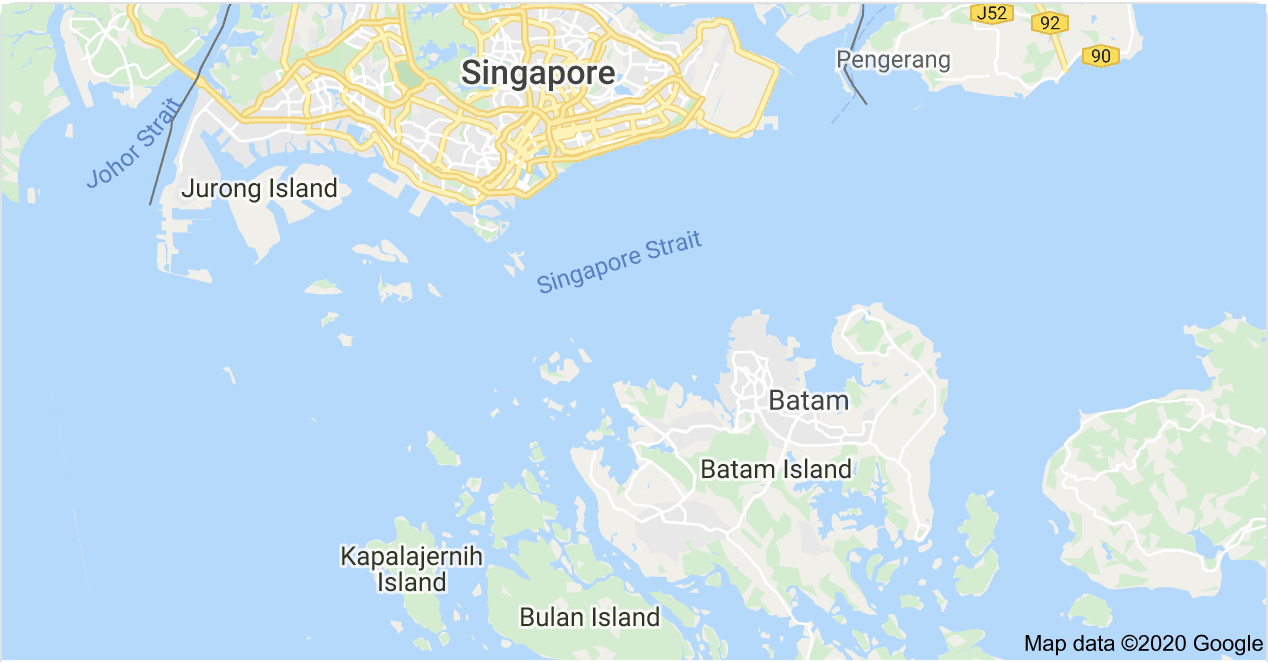
\includegraphics[width=10cm]{pic/ch-eda/sg_straits.png}
    \caption{Singapore Straits Map}
    \label{fig:straits}
\end{figure}

\begin{figure}[t!]
    \centering
    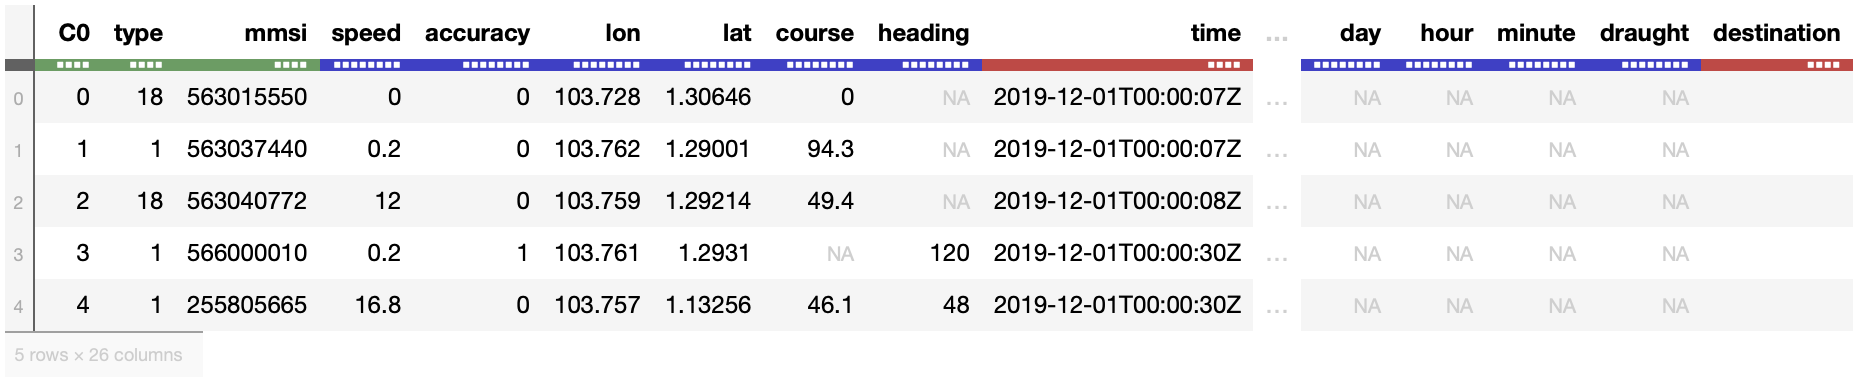
\includegraphics[width=14cm]{pic/ch-eda/overview_ais_records.png}
    \caption{AIS Raw Data}
    \label{fig:records}
\end{figure}

\begin{table}[t!]
    \centering
    \caption{AIS Data Quantity over Class Type}
    \label{tab:table1}
    \begin{tabular}{c|c|c|c}
      \textbf{Class} & \textbf{Position Record} & \textbf{Static Record} & \textbf{Number of Ships}\\
      \hline
      A & 4,151,563 & 203,987 & 26,248\\
      B & 336,202 & 9,058 & 3,443\\
      Total & 4,487.765 & 213,045 & 29,691\\
    \end{tabular}
\end{table}

There are 25 fields currently used by our data center to store AIS records. Some of the fields are erroneous, missing values, and not entirely useful for trajectory analysis either because the fields are hand-updated by humans and hence susceptible to error, or the message sent by the transceiver is not accurate due to faulty sensor. The quality of AIS data is not only critical to the comprehensiveness of analysis but also an essential factor in avoiding misleading prediction results \cite{zhao2018ship}.  We will use several data pre-processing methods proposed by Zhao \emph{et al} \cite{zhao2018ship}. on AIS data and verify the result in the context of our area of interest. The summary of our findings is presented below.

First we will investigate missing values in AIS data. The missing value is defined as the data value that is not stored for a variable in the observation of interest \cite{kang2013prevention}. To identify missing values, we observe the data per class type and compare it within the class. Table \ref{tab:table2} and \ref{tab:table3} summarise missing values by the field for each class of position reports. Class A static report (type 5) does not have a missing values, whilst the only field having missing value in a static report of class B (type 19) is Heading with 97\% proportion. Considering missing values of all class yield the number as shown in Table \ref{tab:table4}. There are 3 fields that suffer from missing values including Speed, Course, and Heading in ascending order.

\begin{table}[t!]
    \centering
    \caption{Missing Values of Class A Position Report}
    \label{tab:table2}
    \begin{tabular}{c|c|c}
      \hline
      \textbf{Field} & \textbf{Missing Values} & \textbf{Proportion}\\
      \hline
      MMSI & 0 & 0.00\%\\
      Speed & 28,788 & 0.70\%\\
      Accuracy & 0 & 0.00\%\\
      Course & 299,701 & 7.21\%\\
      Heading & 1,330,678 & 32.05\%\\
      NavStatus & 0 & 0.00\%\\
      ROT & 0 & 0.00\%\\
      Longitude & 0 & 0.00\%\\
      Latitude & 0 & 0.00\%\\
    \end{tabular}
\end{table}

\begin{table}[t!]
    \centering
    \caption{Missing Values of Class B Position Report}
    \label{tab:table3}
    \begin{tabular}{c|c|c}
      \hline
      \textbf{Field} & \textbf{Missing Values} & \textbf{Proportion}\\
      \hline
      MMSI & 0 & 0.00\%\\
      Speed & 128 & 0.03\%\\
      Accuracy & 0 & 0.00\%\\
      Course & 32,871 & 9.77\%\\
      Heading & 331,764 & 98.67\%\\
      Longitude & 0 & 0.00\%\\
      Latitude & 0 & 0.00\%\\
    \end{tabular}
\end{table}

\begin{table}[t!]
    \centering
    \caption{Missing Values Combined}
    \label{tab:table4}
    \begin{tabular}{c|c|c|c|c}
      \hline
      \textbf{Field} & \textbf{Class A} &\textbf{Proportion} & \textbf{Class B} & \textbf{Proportion}\\
      \hline
      Speed & 28,788 & 0.70\% & 128 & 0.30\%\\
      Course & 299,701 & 7.21\% & 32,871 & 9.52\%\\
      Heading & 1,330,678 & 32.05\% & 340,635 & 98.66\%\\
    \end{tabular}
\end{table}

\begin{table}[t!]
    \centering
    \caption{Erroneous Value by AIS Field}
    \label{tab:table5}
    \begin{tabular}{l|l|l|l}
      \hline
      \textbf{Field} & \textbf{Invalid Criteria} &\textbf{\# Messages} & \textbf{Proportion (\%)}\\
      \hline
      MMSI & Digit's length < 9 & 1,002 & 3.45\\
      ShipType & Undefined & 587,375 & 14.14\\
      CallSign & Non-alphanumeric prefix & 2,750 & 73.41\\
      NavStatus & Undefined & 341,505 & 8.22\\
                & Reserved for future use & 80,974 & 1.95\\
      Longitude & < -180 or > 180 & 21,660 & 0.48\\
      Latitude & < -90 or > 90 & 21,660 & 0.48\\
      Speed & $[102.3, \infty)$ & 0 & 0\\
      Course & $[360, \infty)$ & 0 & 0\\
      Heading & $[360, \infty)$ & 0 & 0\\
      ROT & Undefined & 1428,293 & 34.40\\
      Draught & 0 Length & 12,919 & 6.33\\
    \end{tabular}
\end{table}

The further step of AIS data exploration is to identify erroneous value. One example of an obvious invalid value is longitude with more than 180 and latitude with more than 90. Following Harati-Mokhtari \emph{et al.} \cite{harati2007automatic} recommendation we evaluate the erroneous value of AIS records organized by the AIS field, the result is summarized in Table \ref{tab:table5}. Our findings suggest that erroneous value occupies a small percentage of AIS data. We can mitigate the issue by emitting those values or designing the AIS module system that prevents users from entering invalid values.

\subsection{Trajectory Data Exploration}
\begin{figure}[t!]
    \centering
    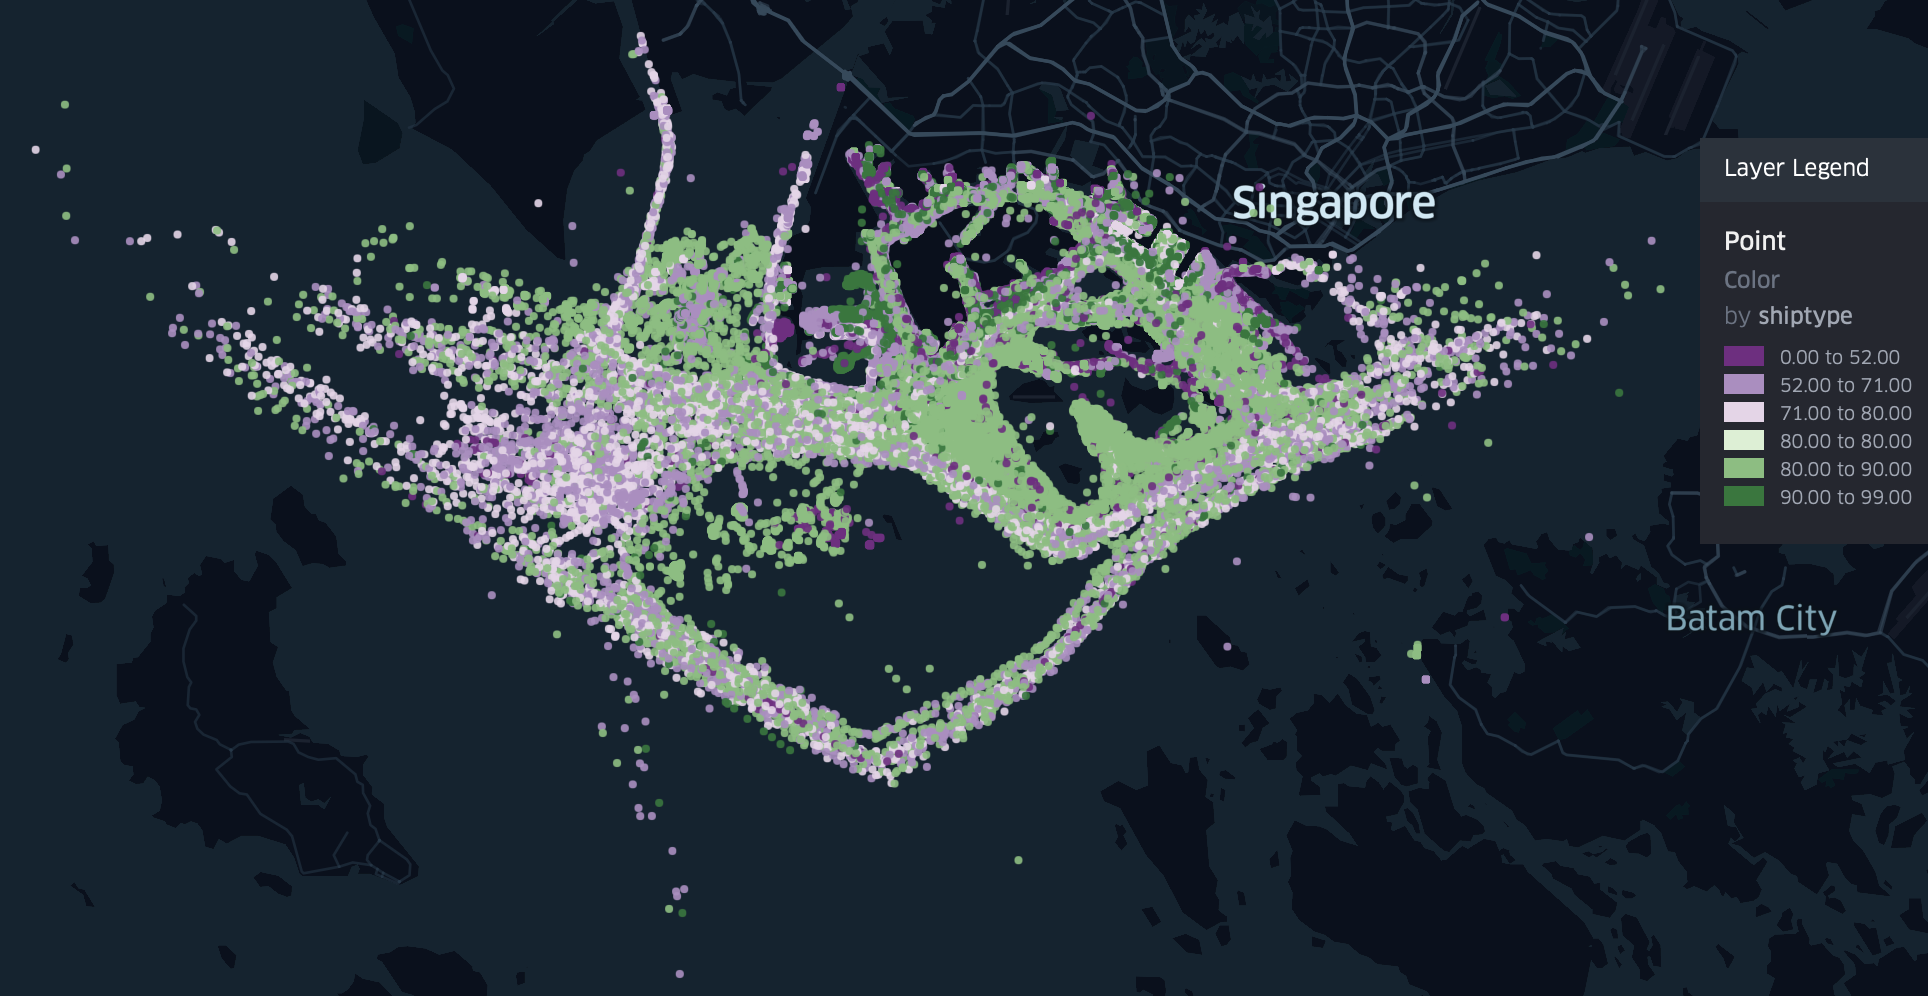
\includegraphics[width=12cm]{pic/ch-eda/overview-legend.png}
    \caption{Vessel Coordinates, generated using kepler.gl}
    \label{fig:traj}
\end{figure}

Figure \ref{fig:traj} is an overview of vessel trajectory over the first seven days of December in Singapore Straits. Trajectory coordinates is plotted using small dots with different color to indicate vessel type. The plot is showing some trajectory patterns, for instance the bottom trajectory is following 'v' letter and is dominated by cargo, tanker, and passengers vessels. It also shows that vessel follows and avoids certain route. A quick look on the trajectory of passengers vessel by using kepler.gl's filter tells us that two common routes being identified are Harbourfront Terminal to Batam Centre and Pasir Panjang Terminal to Bukom Island. We can infer a pattern that vessel from Batam to Harbourfront or the other way shall keep the distance close to Sentosa Island when about to dock or leave Harbourfront terminal.

\begin{figure}[t!]
    \centering
    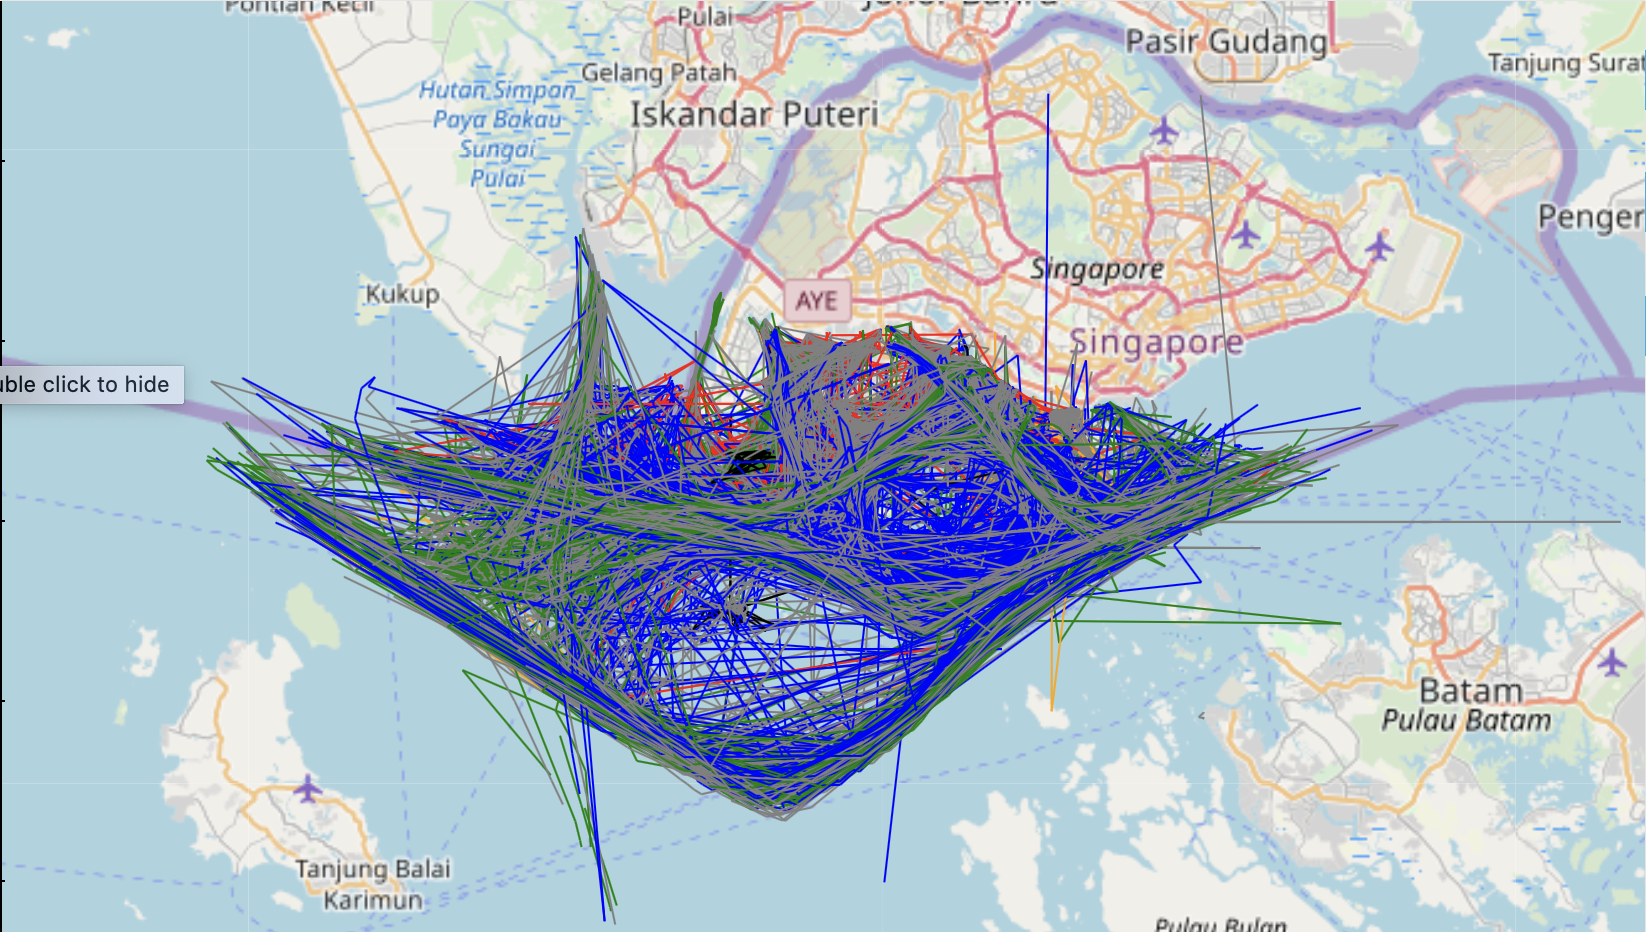
\includegraphics[width=12cm]{pic/ch-eda/trajectories_mpd.png}
    \caption{Coordinates, generated using movingpandas}
    \label{fig:mpd}
\end{figure}

Another way of visualizing vessel movement is to extract a collection of trajectories from datasets per MMSI. Each trajectory is represented by a curved continuous line with different color depending on the ship type. Figure \ref{fig:mpd} confirms similar trajectory pattern with Figure \ref{fig:traj}. The dominating color is green and blue which represents Cargo and Tanker ships respectively. 

AIS records is ideally broadcast by vessel every 2 to 10 second for class A dynamic type message, or every 6 minutes for static type. The AIS dataset we use for exploratory data analysis include dynamic attributes and ship type from static records that is joined by common MMSI. We found that 75\% of dataset have time interval less than 16 minute, while the full interval distribution vary from as close as 0.96 second to as sparse as 6 day. We investigate if the given speed data is rational based on law of psychics. We do this by comparing the original speed with the derived version of speed, computed as distance per time, and then measure the difference. We found that the two version of speed is very close. The number suggest that 75\% of the data differ by less than 0.91. Given the validity of the AIS speed data, we found that about 0.04\% of container ships travel above the average speed of 24 knots, and the maximum recorded speed is 38.6 knots.

\section{Summary}
In this chapter, we discussed about AIS data exploration. All AIS features were demystified, from the definition, decoding the message, to the potential criteria of wrong value. We also explore the dataset using statistics and visualization. First categorize AIS records into two class of A and B. Then we calculate the number of records and unique ships in each class. We also investigate the number of message in all fields with missing and erroneous value according to certain criteria. Finally we conclude the chapter with trajectory exploration by visualizing the first seven week of data.